\documentclass[12pt]{article}
\usepackage{fancyhdr}
\usepackage{hyperref}
\usepackage{float}
\usepackage[margin=0.7in]{geometry}
\usepackage{multicol}
\usepackage{rotating}
\usepackage{lscape}

\usepackage{graphicx}
\pagestyle{fancy}
\graphicspath{{images/}}

\lhead{SET11115 / SET11515}
\rhead{40161642}

\title{SET11108/SET11508 CW}
\author{Rasmus Munk}
\date{\today}
\begin{document}

\section{Introduction:}
This report describes the process of designing and implementing an abstract model in Atelier B and C\# of how a car behaves. This is done by using a combination of classic system design methodologies initally such as a UML model to produce to high level documentation of the system, this is combined with the formal B-Method approach of creating a system with proved correctness/consistency through the use of techniques such as pre and post conditions and invariants that provide proof obligations that can be used to guarantee the correctness of the system. In terms of the outcome car behaviour requirements, the given specification dictated that the car’s controller had to operate under the following conditions:
\begin{itemize}
	\label{list:requirements}
	\item If the engine fails, the brakes must be applied
	\item If the brakes fail, the engine must be stopped
	\item The engine cannot be started without the key being in the ignition
	\item The car cannot increase its speed above a maximum speed limit
	\item If petrol is low a warning light must be shown
	\item If there is a problem with the oil (temperature/pressure) a warning light must be shown
\end{itemize}

In order to provide this car behaviour in an abstract way certain assumptions had to be made. This included that since the aim was to develop an abstract model of how a car behaves a lot of real world specifics were ignored. For instance, the actual logic of how sensors such as the oil, petrol and brake status are actually determined in terms of what constitutes a low petrol level or a high pressure/temperature for oil will not be implemented into this system. The controller/system will instead rely on the state being set by an external system/actor. Furthermore the Driver entity isn't taken into account instead the system is developed from the point of view of the controller. Driver actions are simulated with use of randomly setting the states that the driver could send to the controller via available interface. The content of this report will be presented in the following way. First of the design process of translating the system requirements into an actual system design that lives up to these. This includes creating a UML model followed by the formal definitions, a set of comparisons and between the initial design and the final C\# implementation. Finally an evaluation and conclusion of the final implementation and the process of using correctness development techniques such as the B-Method and Code Contracts to develop an abstract car controller.

\section{UML Design}

In this section the initial transition from the requirements specification to a complete UML model of how the system should be put together will be presented. First up a pair of Use Case Diagrams will be presented, these provide a high level description of what the end system must do and how it will live up to the specification in terms of translating possible user actions into system actions. This is followed by a number of Activity Diagrams that describes the flow control of the car controller to provide the behaviour that is required, for instance the engine can’t be started without the key being in the ignition. Finally, the Class and Sequence diagrams are presented which provide the details on how the system was actually put together and the flow in which the system is executed which provides the required behaviour.

\subsection{Use Case \& Activity Diagrams}
	From the specifications an initial Case Diagram was implemented, this was continuously refined as the system was developed. This initial version of this can be seen \ref{fig:use1}.
	
	As \ref{fig:use1} shows the actions are launched by the interactions Driver shown in the left side of the diagram. This entity has a number of actions that can be performed, all of which are in captioned in the “Driver Interface” sub system. This includes inserted/withdrawing the key, applying and releasing the accelerator and brake pedals. These different actions are transmitted to the “Car Controller” who is responsible for “executing” those actions in accordance with the specs specified. For instance, when the key is inserted the controller registers this and instructs the “Engine Interface” subsystem to turn on the engine via the Start Engine action. As mentioned in the introduction the logic for setting a state is decided by the external actor’s such as the Petrol Sensor, Oil Sensor, Speedometer etc. An example of design refinement can be seen in \ref{fig:use1} where it does not include actions such as release brakes. The reason for this was that the Drivers action should of course be translated into an internal brake status change.
	
	\begin{sidewaysfigure}
			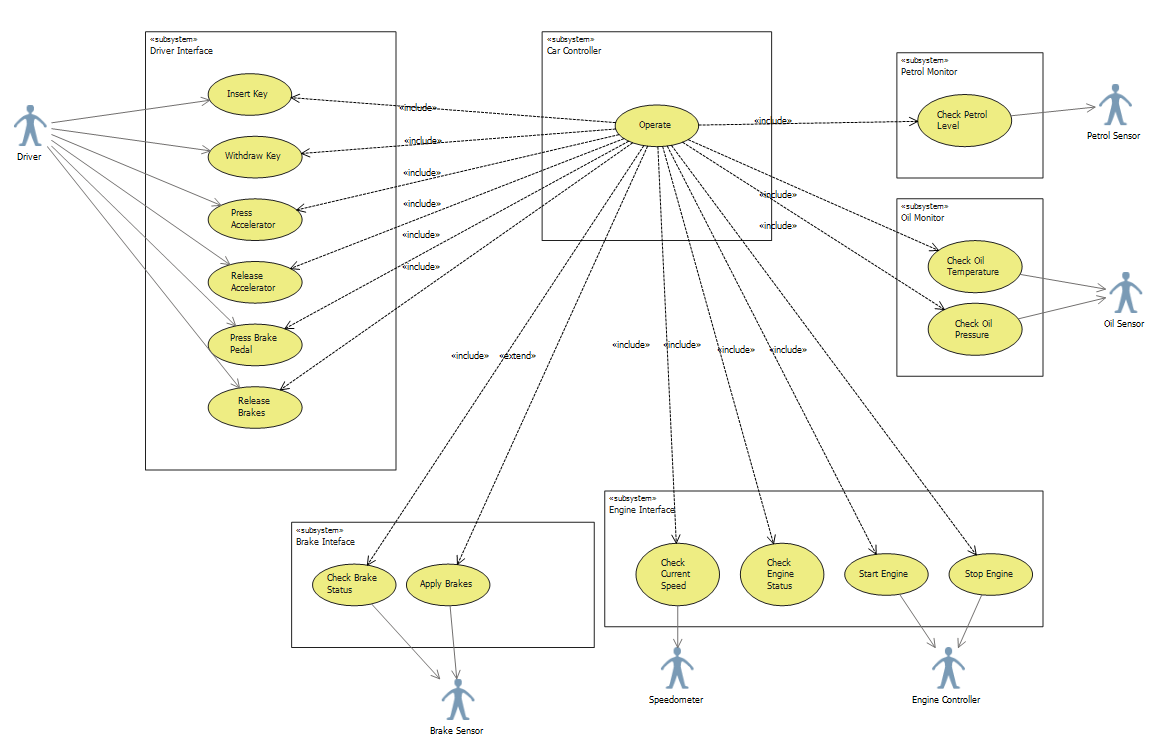
\includegraphics[width=0.8\textwidth]{use_case_diagram_v1}
			\caption{Use Case Diagram v1}
			\label{fig:use1}
	\end{sidewaysfigure}

From this initial use case diagram an activity diagram was created to show the flow of the car controller behaviour. As with the use case diagrams this was also continuously refined, the final version of this process can be seen from \ref{fig:act1} to \ref{fig:act4}.

\begin{figure}[H]
	\centering
	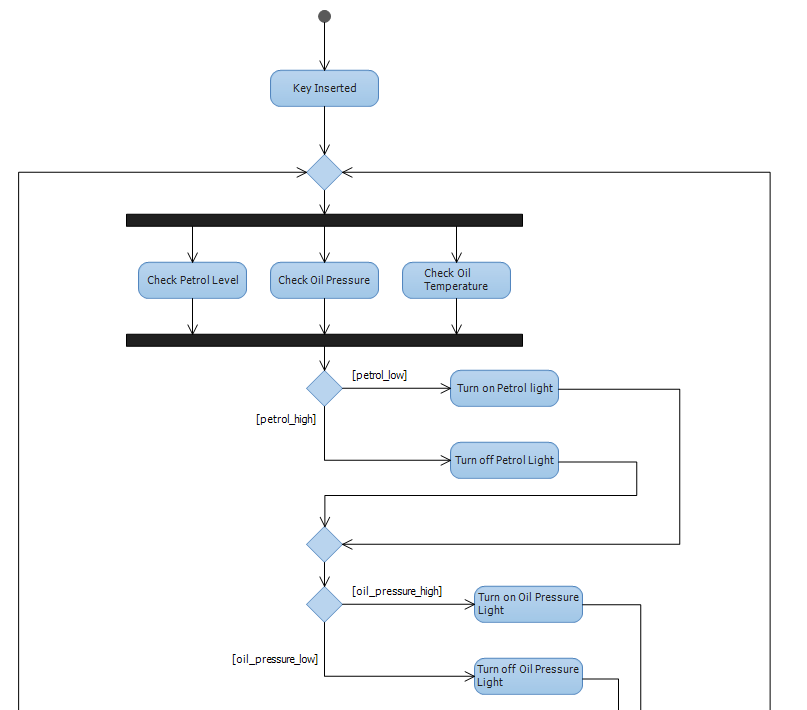
\includegraphics[width=0.6\textwidth]{activity_diagram_v1}
	\caption{Car Controller Final Activity Diagram 1-4}
	\label{fig:act1}
\end{figure}

As the activity figures display the execution of the car controller’s operation loop relies on whether the key has been inserted or not, before this happens the controller won’t perform any other action than continuously checking whether the key has been inserted. If this ever happens the controller then continuous to retrieve the Oil and Petrol states and based on these make a decision on whether to turn on a warning light for that state, as shown in \ref{fig:act2} if the Oil Temperature is High it turns on the Oil Temperature Light as specified in the requirements. From this the controller moves on to evaluate whether the engine should be turned on or not, checking the states of the pedals brakes and engines and based on these and the current state decide whether the engine should be turned off, brakes should be applied or the speed should be increased as shown in \ref{fig:act3}.

\begin{figure}[H]
	\centering
	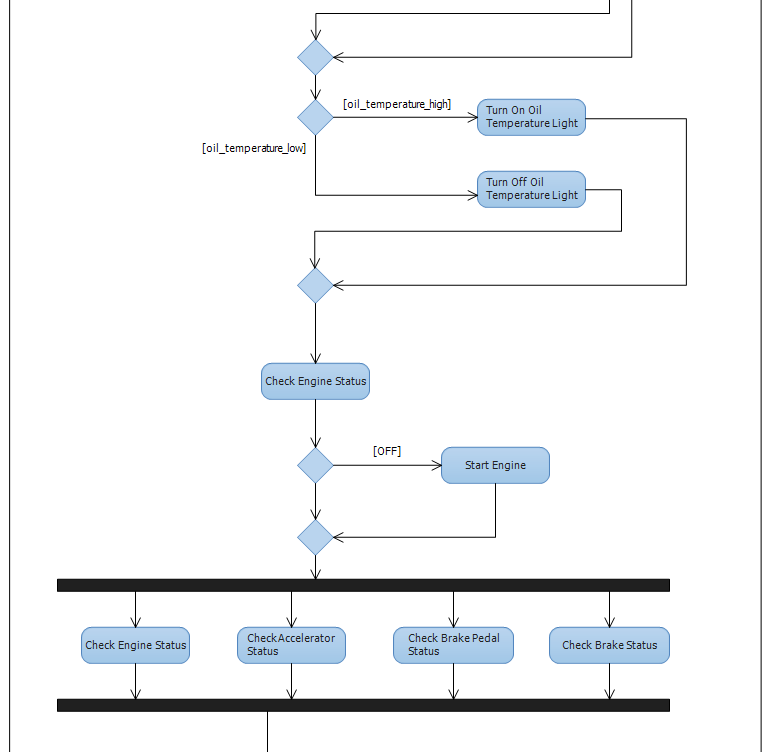
\includegraphics[width=0.6\textwidth]{activity_diagram_v2}
	\caption{Car Controller Final Activity Diagram 2-4}
	\label{fig:act2}
\end{figure}


\begin{figure}[H]
	\centering
	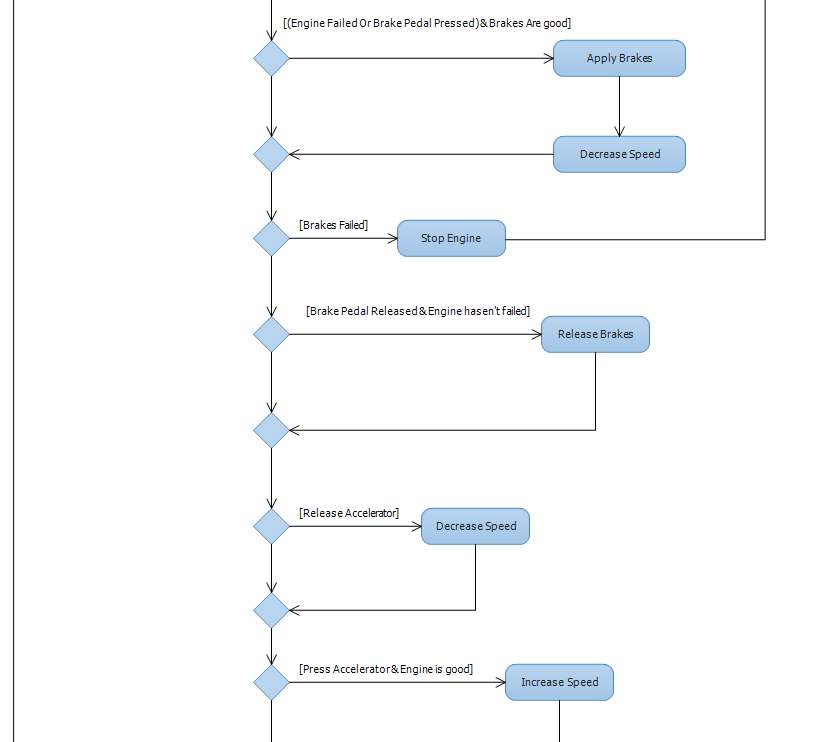
\includegraphics[width=0.6\textwidth]{activity_diagram_v3}
	\caption{Car Controller Final Activity Diagram 3-4}
	\label{fig:act3}
\end{figure}

\begin{figure}[H]
	\centering
	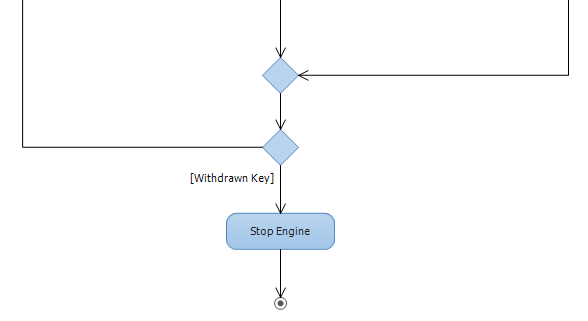
\includegraphics[width=0.6\textwidth]{activity_diagram_v4}
	\caption{Car Controller Final Activity Diagram 4-4}
	\label{fig:act4}
\end{figure}

\subsection{Class and Sequence Diagrams}

As indicated the all of the different design aspects have gone through several changes throughout the development. An example of this will be shown in the following section where the initial class and sequence diagrams can be seen in \ref{fig:class1}, \ref{fig:class2}, \ref{fig:seq1} and \ref{fig:seq2}.


\begin{figure}[H]
	\centering
	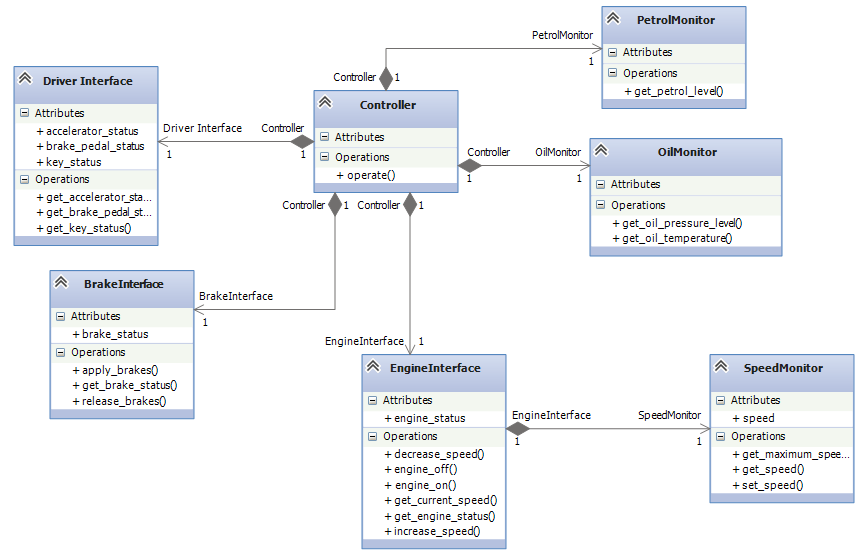
\includegraphics[width=0.8\textwidth]{class_diagram_v1}
	\caption{Class Diagram v1}
	\label{fig:class1}
\end{figure}

As can be seen the initial class, it was expected that all of the driver states would be contained in the “Driver Interface” class. However, this is not correct since the specification dictates that these actions were supposed to be separated into 3 separate classes, these were the Pedals, Dashboard and Ignition classes as can be seen in \ref{fig:class2}. Furthermore, as the figure also shows the functionality to control the warning lights was also added through the Dashboard class. This would work by passing a set of warning to the emit\_warning\_states() method which then would decide whether to turn on a particular state dependent on the passed states. 

\begin{figure}[H]
	\centering
	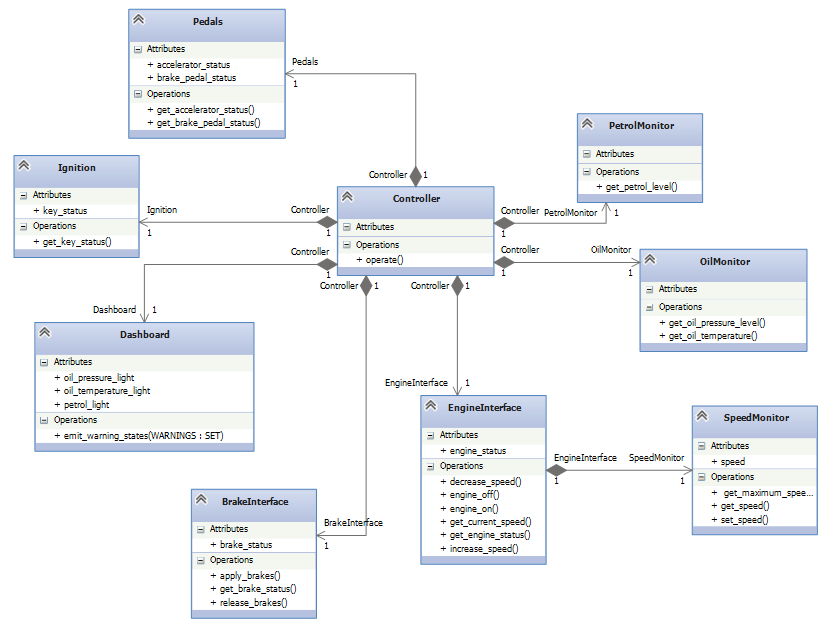
\includegraphics[width=0.8\textwidth]{class_diagram_v2}
	\caption{Class Diagram v2}
	\label{fig:class2}
\end{figure}

The changes to the class diagram design was carried forward to the sequence analysis as can be seen in \ref{fig:seq1} and \ref{fig:seq2}. These diagrams lay out the specific communication there is expected to take place between the system components. The instigator of these series of events is the Controller class which queries the other components for information about their current state. Based on the returns the Controller then executes a specific action. e.g. The OilMonitor returns that the temperature is high which means that the Controller instructs the Dashboard that it should turn on the oil temperature warning light. 

\begin{landscape}
	\begin{figure}[H]
		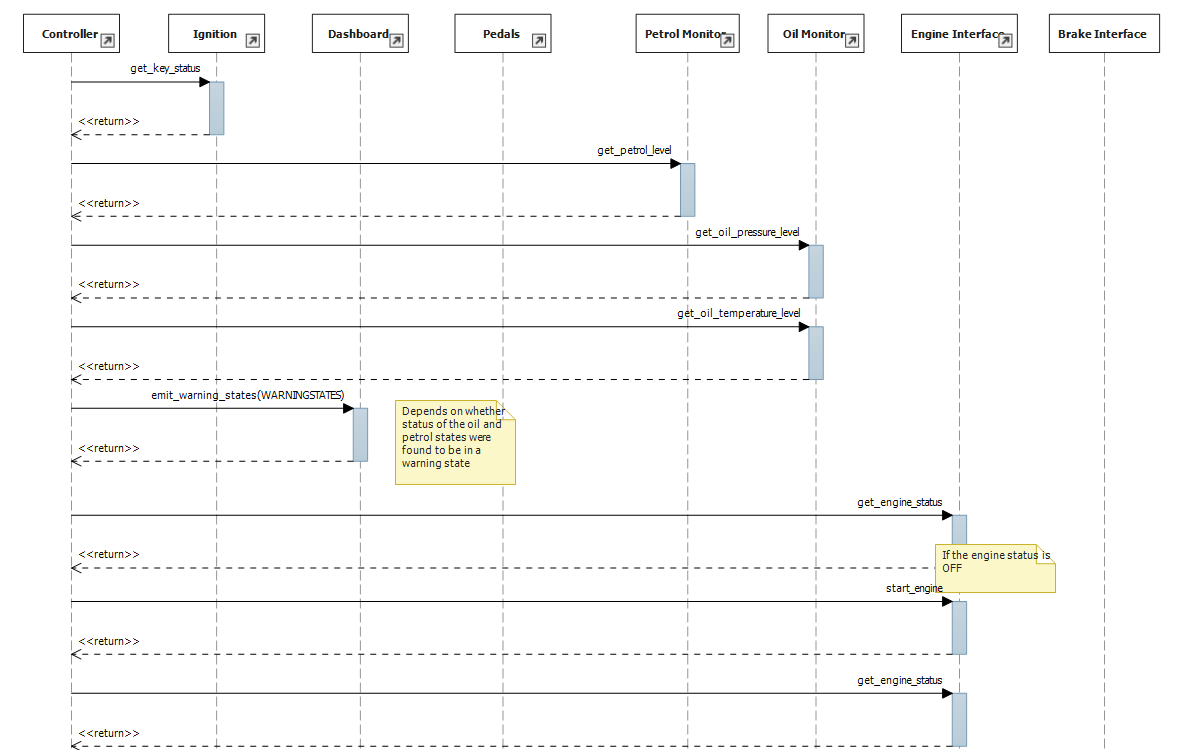
\includegraphics[width=1.2\textwidth]{sequence_diagram_v1}
		\caption{Sequence Diagram 1-2 v1}
		\label{fig:seq1}
	\end{figure}
\end{landscape}

\begin{landscape}
	\begin{figure}[H]
		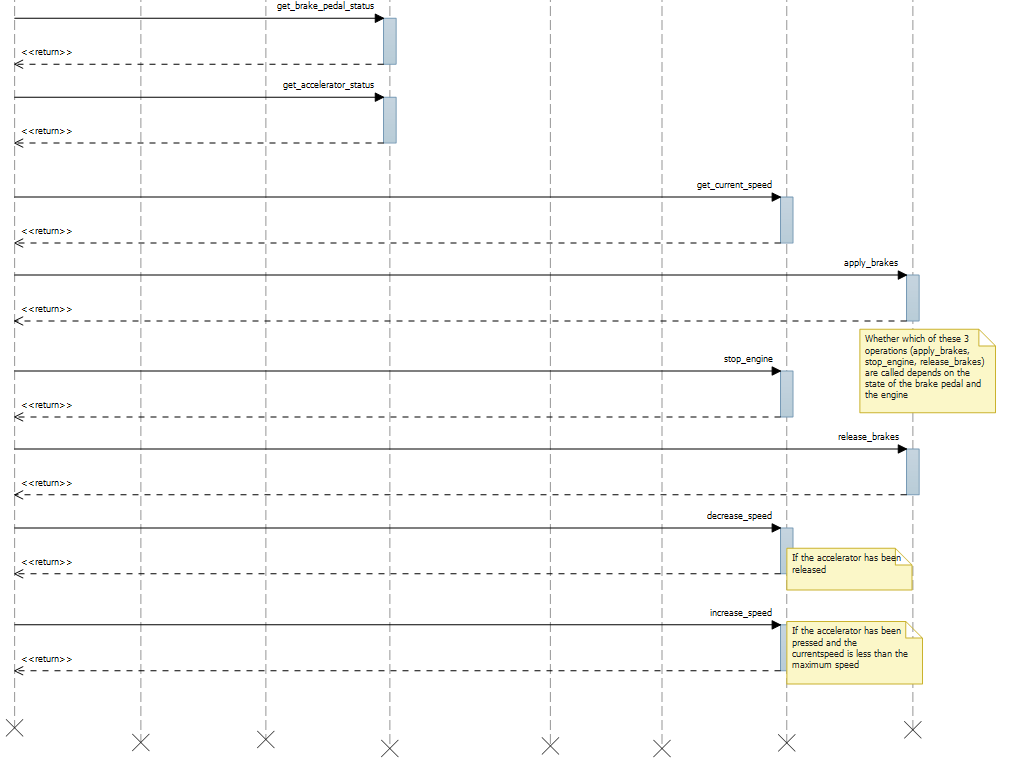
\includegraphics[width=1.2\textwidth]{sequence_diagram_v2}
		\caption{Sequence Diagram 2-2 v1}
		\label{fig:seq2}
	\end{figure}
\end{landscape}

In summary, the initial specifications were translated from a set of requirements to a concrete set of use cases which displays the functions that the system should be able to perform to fulfil the requirements. Furthermore, an activity diagram was developed to that shows the high-level flow control of the car controller that provides the required abstract behaviour of how the state changes should affect how the car operates, e.g. if the engine fails the brakes must be applied. Furthermore, the initial class and were presented including how they changed from an initial contained driver interface to separate dashboard pedals and ignition components. Finally, the sequence diagrams described how the proposed components are expected to interact with the controller as the main class that will act based on the responses.

\section{B Method}

In this section the B-method definitions for the system design will be presented. An initial overview of the different machines implemented can be seen in \ref{fig:bmethod1}.

\begin{figure}[H]
	\centering
	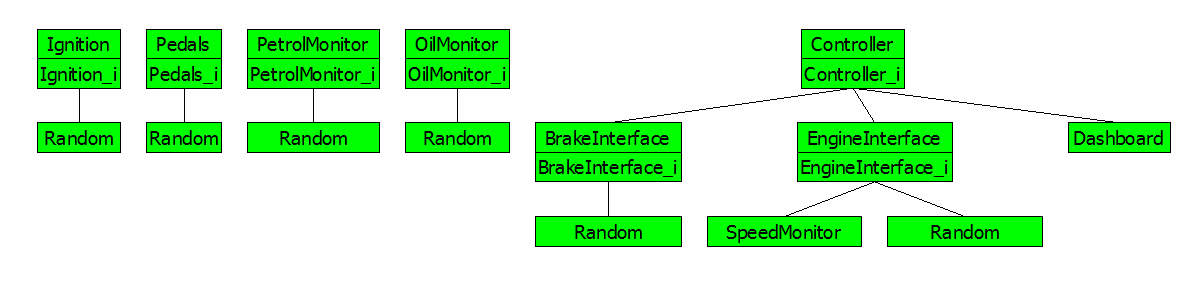
\includegraphics[width=1.0\textwidth]{machine_overview_v5}
	\caption{Machine Definitions}
	\label{fig:bmethod1}
\end{figure}

As this shows, the B-method implementation is highly based on the class and sequence diagram. In that the same names/classes are created separately but are implemented in the Abstract Machine Notation(AMB) format in Atelier B. However, a difference is that some of the abstract machines utilizes refinement to provide a concrete implementation of how an operation should be performed, whereas the overlying definition only provides details on what this operation does or what it is supposed to return. This is different compared to the class diagram where it is illustrated as each class/machine implements the operational logic on its own. An example of this can be seen with the BrakeInterface or the EngineInterface machines as shown from \ref{fig:bmethod2} to \textbf{Figure xx.}


\begin{figure}[H]
	\centering
	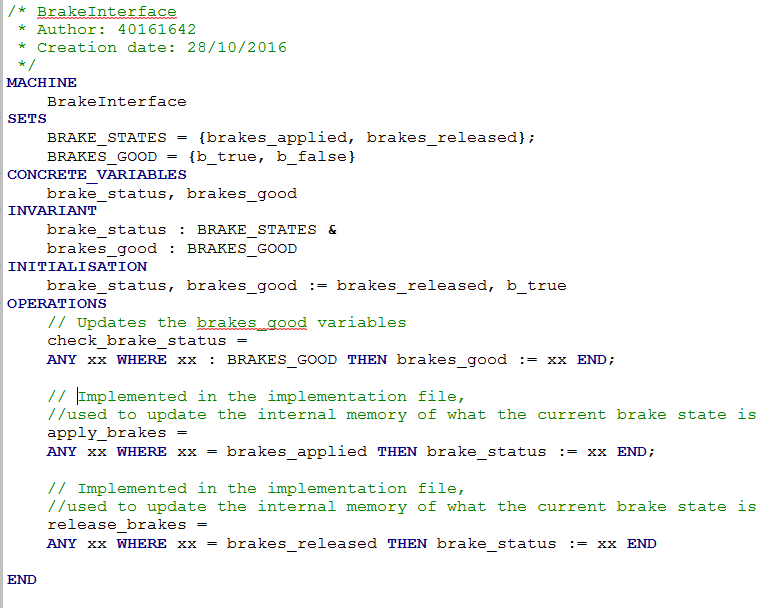
\includegraphics[width=0.8\textwidth]{brake_interface}
	\caption{BrakeInterface Abstract Machine}
	\label{fig:bmethod2}
\end{figure}

Here the abstract machine defines that the operation \textit{check\_brake\_status} that updates the \textit{brakes\_good} variable. Which of these states are returned and how a state is selected the abstract operation doesn’t care about instead if defines the states that the caller of this operation can expect to receive. Instead it is the implementation machine’s responsibility to defined which state is returned, a similar design approach is used across the Ignition, OilMonitor, Pedals, PetrolMonitor whereas instead of defining concrete variables in the interface or the implementation machines the internal machines only return values without updating an internal state. The reason for this was that the decision for the return value in these cases doesn’t rely on the history of which values have been returned before. E.g. the PetrolMonitor machine should just switch between returning \textit{petrol\_low} or \textit{petrol\_high}. However, in this design setup it is up to the caller to save the value that these machine operations return. i.e. the Controller in this case. Also because the machines have no internal state the Controller can be sure that there won’t be any internal state changes and can function with seeing the machines instead of importing them. 
Beyond this the only exception in terms of design is the Dashboard machine where there is only a concrete machine and no interface, the reason for this exception was that because of the requirements the caller should be able to directly set the state for this machine, e.g. turn on the petrol warning light when the PetrolMonitor returns the \textit{petrol\_low} state. In terms of Atelier B this does require that the Controller import this to read the internal variable state of this machine.
In terms of how the implementation machines are implemented, an example of this can be seen with the BrakeInterface\_i machine in \ref{fig:bmethod3}. This shows that when a caller executes the operation \textit{get\_brake\_status} the operation makes a coin flip decision between either updating the brakes to have failed or just returning the previous set state. It does this by requesting a random value of either 1 or 0 from the imported Random machine operation \textit{get\_random\_value}. 

\begin{figure}[H]
	\centering
	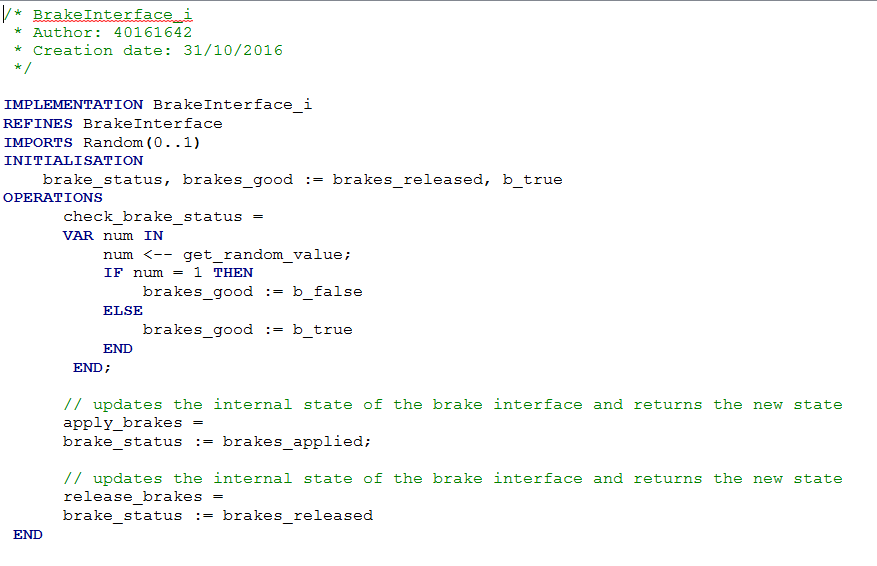
\includegraphics[width=1.0\textwidth]{brake_interface_implementationv2}
	\caption{BrakeInterface Implmentation Machine}
	\label{fig:bmethod3}
\end{figure}

Another example would be the EngineInterface machine where the base abstract machine defines 6 abstract operations as shown in \ref{fig:bmethod4}. As before, each of these dictates what the operation can return, change or accept as input in form of the preconditions. To handle how these are executed the EngineInterface\_i machine defines this as can be seen in \ref{fig:bmethod5} and \ref{fig:bmethod6}.

\begin{figure}[H]
	\centering
	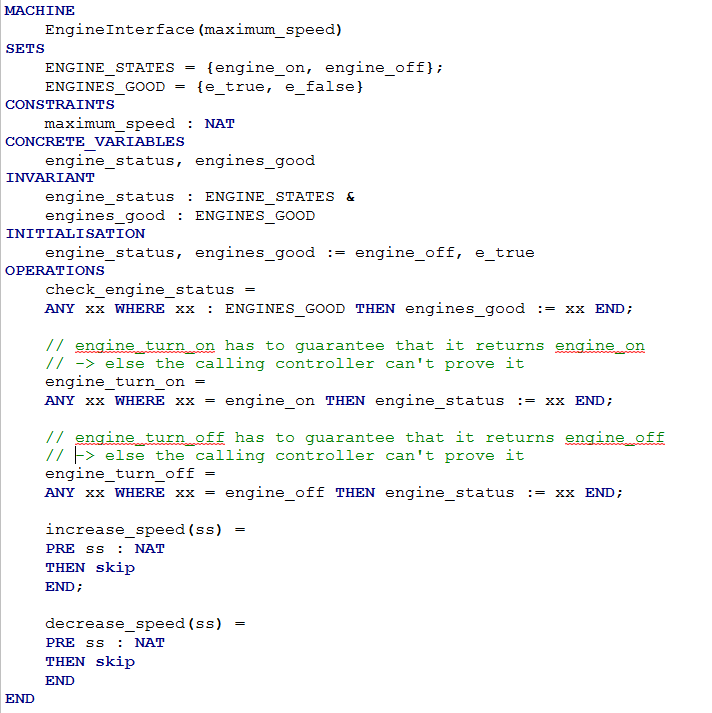
\includegraphics[width=0.8\textwidth]{engine_interface_abstract_v2}
	\caption{EngineInterface Abstract Machine}
	\label{fig:bmethod4}
\end{figure}

As shown in \ref{fig:bmethod4} the EngineInterface base machine defines two concrete state variables. The reason for this was that the Controller would then have direct read access to the state of these and therefore wouldn’t be required to define local variables to track the state of this machine. The approach was also applied to the BrakeInterface base class as can be seen in \ref{fig:bmethod2}.

This approach of using internal state variables was the initial approach across a number of machines including Pedals, PetrolMonitor, OilMonitor and the Ignition machine. An example of the specific OilMonitor machine can be seen in \ref{fig:bmethod7}. Here the concrete variable \textit{last\_pressure\_state} and \textit{last\_temperature\_state} are used to determine what the states will become next by calling the either operations. However, this approach was abandoned because it would mean the initialisation state of the two variables would determine the continuous pattern of these two. E.g. when the temperature is high the pressure is low or the opposite or both are low and then high. To avoid the deterministic state behaviour the implementation was changed to utilize the same Random machine approach as with the Brake and EngineInterface machines. This new design approach can be seen in \ref{fig:bmethod8}. This was then also applied to the Pedals, PetrolMonitor and Ignition machine as shown in \ref{fig:bmethod1}.

\begin{figure}
	\centering
	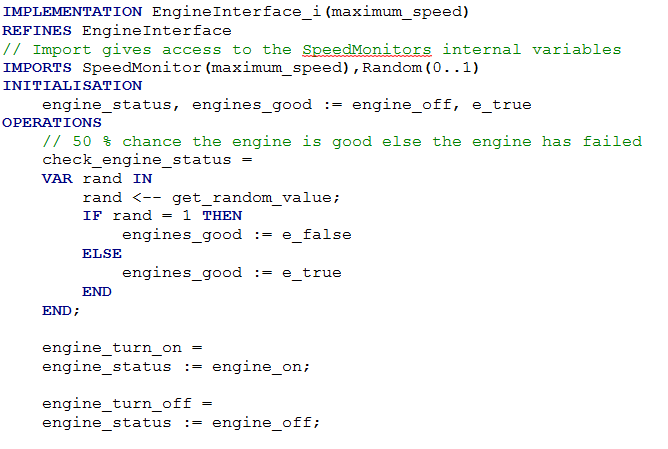
\includegraphics[width=0.7\textwidth]{engine_interface_implementation_v2_1}
	\caption{EngineInterface Implementation Machine }
	\label{fig:bmethod5}
\end{figure}

\begin{figure}
	\centering
	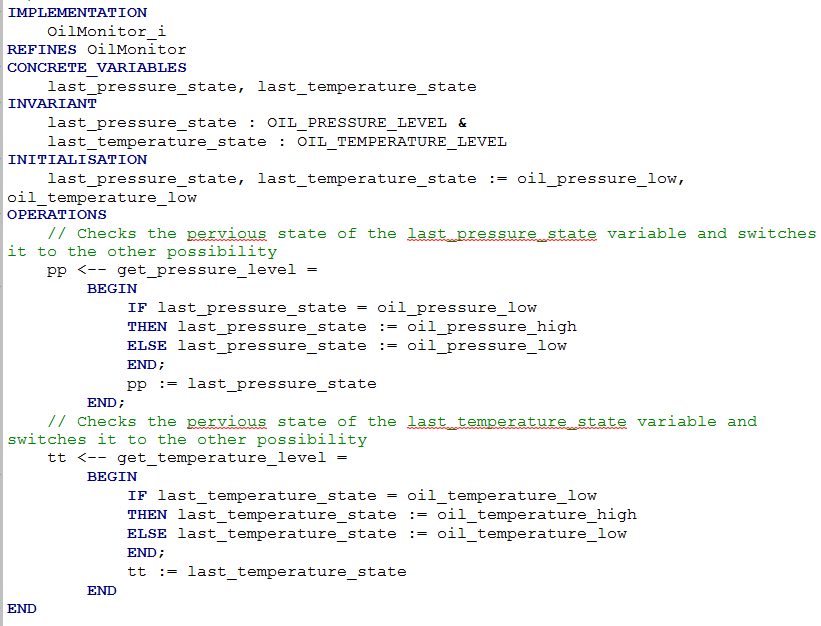
\includegraphics[width=0.8\textwidth]{previous_oil_monitor}
	\caption{Previous OilMonitor Implementation}
	\label{fig:bmethod7}
\end{figure}

\begin{figure}
	\centering
	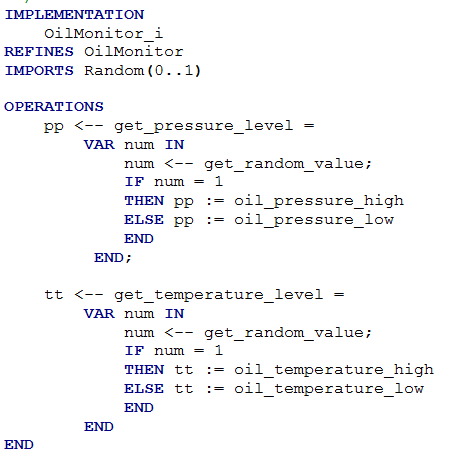
\includegraphics[width=0.5\textwidth]{current_oil_monitor}
	\caption{Current OilMonitor Implementation}
	\label{fig:bmethod8}
\end{figure}

Beyond the development changes described to the implemented machines several other deviations occurred from the initial UML design. An example of this is that the Dashboard machine changed from the initial idea of using the operation \textit{emit\_warning\_states} to control which lights would be on or off. It would do this by taking a set of warning states as a parameter, based on these the Controller would set the appropriate state for the various lights in Dashboard machine. Specifically, it was attempted to make update the internal light states by overwriting the internal state set with the passed in WARNINGS set. This however would require that the controller on each operate call to declare a warning states set and translate the current petrol and oil states into appropriate dashboard light state for each call of these before passing it to the dashboard operation. Instead of this, it would be simpler to just check the petrol and oil states in the Controller and update the internal dashboard state variables by calling a specific operation for that light. The specific implementation of this can be seen \ref{fig:bmethod9} and how it is called in the controller in \ref{fig:bmethod11}.

\begin{figure}
	\centering
	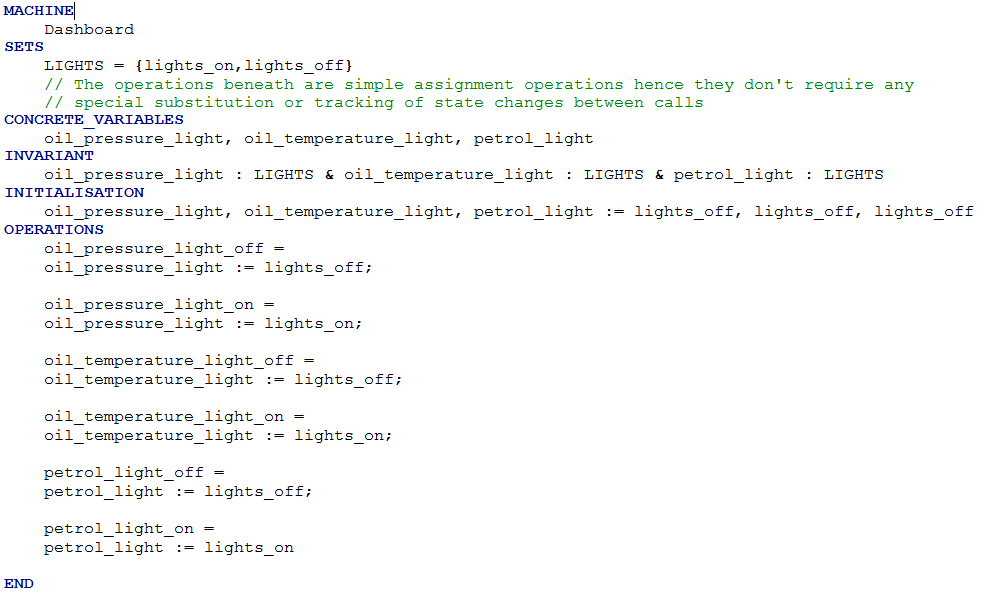
\includegraphics[width=0.8\textwidth]{dashboard_implementation}
	\caption{Dashboard Machine}
	\label{fig:bmethod9}
\end{figure}
Overall the machine design as shown in \ref{fig:bmethod1} contrasts to the initial class diagram in \ref{fig:class2}. In the class diagram, each of the components e.g. Pedals, Ignition are separated into their own concrete classes. This contrasts with the B-Method design in \ref{fig:bmethod1}, here every controller except for the Dashboard and the SpeedMonitor are separated into an abstract interface and a refined implementation. The reason for this was that it enabled helpful features in the concrete implementations, such as support for local variable substitution in the \textit{check\_engine\_state} in \ref{fig:bmethod5}. In order to store a random number in the operation call from the Random machine \textit{get\_random\_value} operation.

This contrasts with the class diagram where each component/class is included into the controller via association by either passing an instantiation of a particular object to the controller or the controller instantiating it. What this separation of concrete classes into abstract machines and concrete implementation files provides, is that it makes the implementation ready for changes in the future, e.g. if the way in which the BrakeInterface returns a state changes it should be able to restrict the code modifications to the BrakeInterface implementation itself. A downside to this approach is that when the controller imports/sees these abstract machines it has to extract the state of that refined machine through its operations since it doesn’t have direct read access to the implementation machines concrete variables. A workaround to this is to declare concrete variables in the base class machine as was used in the Brake and EngineInterface machines.

It should be noted that there are certainly other ways the system could have been designed, however in this instance it seemed adequate because it provided the functionalities/operational behaviour that was required by the specification as highlighted in \ref{list:requirements}. In terms of  controller behaviour including the specific state invariants, the final implementation of this can be seen from \ref{fig:bmethod10} to \ref{fig:bmethod12}. From the flow of this controllers operate operation, it follows the lines layed out in the activity and sequence diagrams. e.g. the controller first checks the oil/petrol states, hereafter it checks the accelerator pedal, brake pedal, brake and engine status. Based on the state these check returns the controller decides which action the car should execute, e.g. apply brakes or increase/decrease speed or turn the engine off due to the brakes have failed. Although some notable changes include the mentioned change from not using the \textit{emit\_warning\_state()} to separately call the specific Dashboard operation that either turns on or switches off a particular light.

\begin{figure}[H]
	\centering
	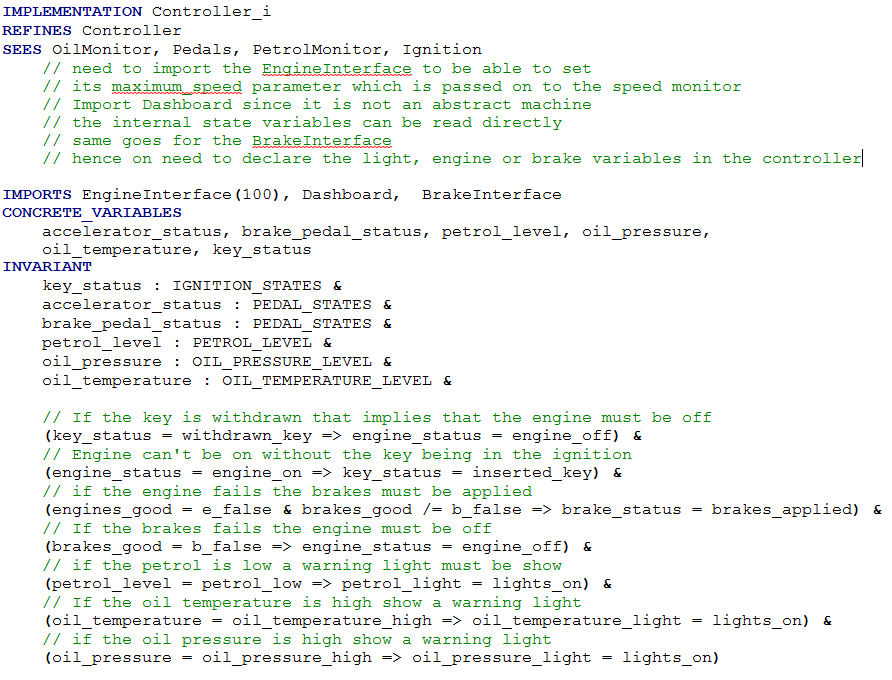
\includegraphics[width=0.8\textwidth]{new_controller_v1}
	\caption{Final Controller 1-3}
	\label{fig:bmethod10}
\end{figure}

\begin{figure}[H]
	\centering
	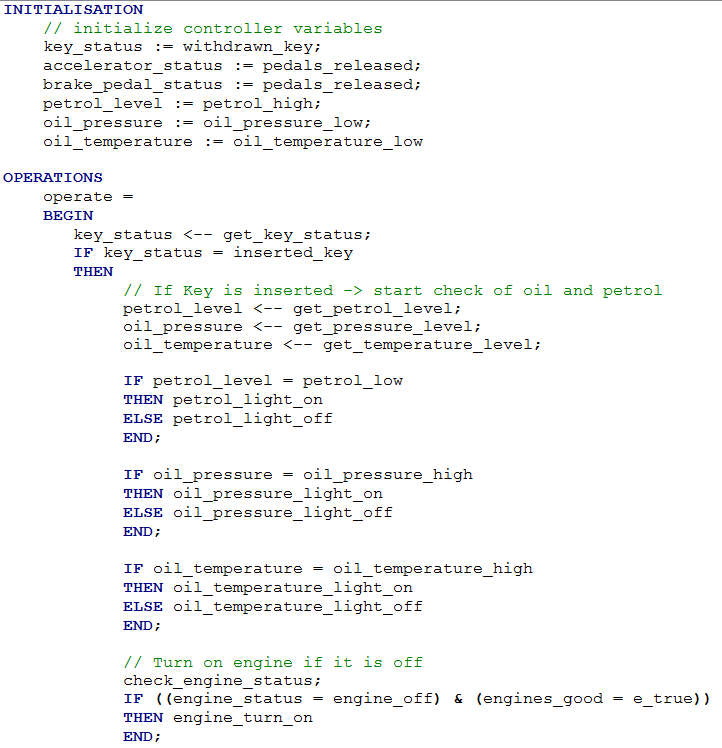
\includegraphics[width=0.6\textwidth]{new_controller_v2}
	\caption{Final Controller 2-3}
	\label{fig:bmethod11}
\end{figure}

\begin{figure}[H]
	\centering
	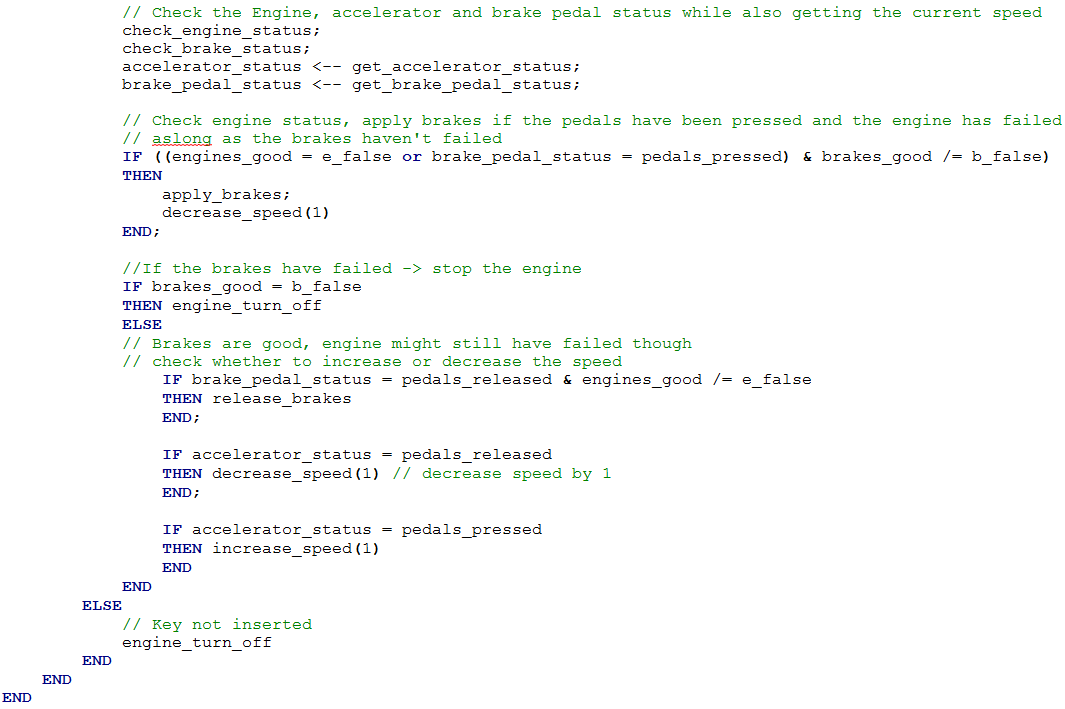
\includegraphics[width=0.8\textwidth]{new_controller_v3}
	\caption{Final Controller 3-3}
	\label{fig:bmethod12}
\end{figure}

In terms of proof obligations for the machines highlighted in \ref{fig:bmethod1} the confirmation that these are not violated can be seen in \ref{fig:bmethod13}.

\begin{figure}
	\centering
	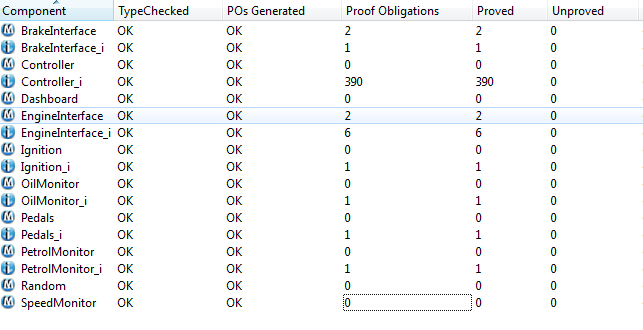
\includegraphics[width=0.7\textwidth]{proof_obligations_v2}
	\caption{Proof Obligations}
	\label{fig:bmethod13}
\end{figure}

As \ref{fig:bmethod13} shows the B-method implementation fulfil all the proof obligations that are defined by the system invariants. A bit surprising is that the Controller implementation has 390 proof obligations, a reason for this could be that since the speed aspect was implemented as a natural number no bigger than the number in which the EngineInterface is instantiated with which in this case was 100 is likely the cause for this bloat in proof obligations.

\section{Final Implementation}

The final implementation consists of a C\# implementation of classes and Code Contracts that are directly based on the initial design and the presented B-method specification.


To enforce the correctness of the B-Method design a  number of CC capabilities were used including invariants on the class definitions, preconditions on the entry of method calls and post conditions to ensure the caller of the object state after the method call has finished. An example of this can be seen in \ref{fig:cc1} where a postcondition ensures the caller that after the method \textit{oil\_pressure\_light\_on()} has finished the Dashboard state of the \textbf{oil\_pressure\_light} has switched to on.
\begin{figure}[H]
	\centering
	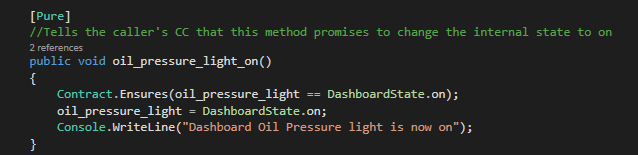
\includegraphics[width=0.7\textwidth]{cc_ensures_dashbord}
	\caption{Dashboard Turn on the Oil Pressure Warning}
	\label{fig:cc1}
\end{figure}

Furthermore because this call is executed by the controller through an instantiated dashboard object the internal method has to tell the controller that beyond the visible changes no further changes will be made to the observable state. This is where the [Pure] declaration comes into play, because it is exactly what it provides to the analyser. However this indication comes with no guarantee in that no error will be displayed if the method in face would change the internal state of the dashboard object.

This example is a good indication of how the final implementation was developed. It consisted of translating the functionality/structure of the B-Method and initial class diagrams into a set of classes that provide the exactly same functionality through as little deviation as possible.

To prove that this implementation behaves as the requirements state a number of unit tests were implemented. 

What these tests cover includes e.g. the FailToGoAboveTheMaximumSpeed that increases the speed above the maximum defined speed and validate whether the speed isen't above the maxmimum speed. Another example includes whether the CC will throw an exception if the engine is left on after the brakes have failed i.e. the FailRunningEngineWhenBrakesFailed test as shown in \ref{fig:cc2}.

\begin{figure}[H]
	\centering
	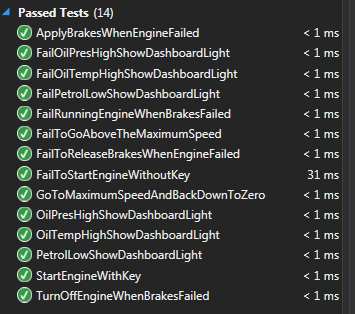
\includegraphics[width=0.4\textwidth]{cc_tests}
	\caption{System Tests}
	\label{fig:cc2}
\end{figure}

\section{Evaluation of the Final Implementation}

All in all the final implementation delivers a fully functional abstract car system implemented with Code Contracts(CC) in C\#. This implementation is highly identical to the B-Method specification of machine definitions and how they communicate with each other. e.g. the system utilizes a main Controller that is being passed instantiations of the machines it sees from a CarSystem object. Beyond this it itself handles the creation of the imported machines i.e. the Engine/BrakeInterface and the Dashboard object.

 Furthermore, to validate that this implementation works as required a series of tests were implemented. As \ref{fig:cc2} shows these all passed by returning the value that was expected. This in addition to the B-Method specifications shows that the implemented system provides the required behaviour while delivering it with proved correctness and consistency. In terms of the Code Contracts the analyser proved to be unable to tell the state of an internal variables of an owned instantiated object. This resulted in a number of warnings about the possibility of the system being unproven because it couldn't verify the state of these. To get around this the variables could either be made public so they could be verified or the analyser had to be told what state it could expect after an arbitrary method call. To enable this the implementation strongly utilizes these CC capabilities to tell the analyser what it could expect.


\section{Conclusions}

In conclusion, the developing of an abstract car system included an initial UML design consisting of Use Case, Activity, class and sequence diagram to gather an initial layout to how the proposed system should be implemented. This initial approach was used to produce a B-Method specification with a number of abstract/implementation machines as can be seen in \ref{fig:bmethod1}. This specification provided a foundation to how the system could be designed while upholding correctness and consistency by abiding by the invariants/proof obligations imposed on the system. Out of these 405 proof obligations everyone of them passed proving that this design would provide the specified behaviour. This in turn was used as a structure to implement a C\# implementation of this specification that makes it possible to simulate the behaviour of this system through a console application that has been verified by a number of unit tests as shown in \ref{fig:cc2}.

In terms of the B-method approach enables the software developer to prove correctness of his/her design. This means that it is guaranteed that the system will not end up in a state that has not been allowed by the specifications rules/invariants. The approach does however not guarantee that the end behaviour of the system is as expected. For instance the invariant only states that the car should turn off the engine when the brakes fail and doesn't specify whether the brakes should be allowed to "unfail" the execution could be stuck in that the brake state will never change, hence that the engine will be turned off whenever it is started. This means that the approach doesn't allow the developer to just implement the design an then be contempt because it dosen't brake the preconditions and the specified invariants. It is still the task of the developer to make sure that the behaviour is as required. To cover this simple tests methods could be applied to identify any problems in this area. 

In terms of Code Contracts it provides a method to validate the correctness in a real application by utilizing capabilities such as Invariants, Requires and Ensure methods to validate the state of objects in terms of their internal variables. This process is useful for systems like a car controller where safety is important because a program bug could result in the loss of life in the worst instance. Therefore it is important to being able to ensure the consumer/company that the system is guaranteed to never reach an unwanted state, as long as these boundaries have been defined correctly.


\bibliographystyle{plain}
\bibliography{/Users/rasmusmunk/Documents/Bibtex/library.bib}

\end{document}